\chapter{Image manipulation}
\vspace{-10mm}

Dicom-Presenter is an application for viewing image data. Entire image manipulation was solved with use of OpenGL library in early version of Dicom-Presenter. OpenGL was used for image storing, for changing image properties and for drawing images on screen. Unfortunately, OpenGL brought complications to application compatibility with various hardware. Therefore, author of this work decided to remove OpenGL from application and replace all classes using OpenGL with their non-OpenGL equivalents. 

Before rewriting all image processing classes without OpenGL it was a need to study how to complete all image processing tasks without OpenGL. Moreover, OpenGL uses GPU to perform it's tasks so it was a need to calculate the loss of performance when OpenGL will be removed. 

\section{Image storing}
\label{rawdata}
There are two different libraries used for image manipulation in Dicom-Presenter. DCMTK library is used for loading images from hard disk, while Qt library (formely OpenGL) is used for displaying images on computer screen. DCMTK library must be used since it supports loading files in DICOM format, besides some application framework must be used for image displaying. DCMTK library offers loading compressed image files and saving them uncompressed into RAM memory. To be able to display these raw data properly by Qt library, it is mandatory to understand the way image data are represented in computer. 

A color image consisting of $m \cdot n$ points (pixels) can be described by $m \cdot n$ number triads. The triads would be coordinates in RGB or HSV color space \footnote{Colors which can be displayed can be fully described by three values. This fact is based on human eye anatomy and leads to construction of coordinate systems describing each displayable color. Coordinates of RGB color space are red, blue, green color while hue, saturation, value are coordinates in HSV color space.}. Data in a computer are stored in elementary units - bytes, which can hold 256 different values. Each byte consists of eight unitary units - bits ($2^8 = 256 $). If considered that one byte can include color information of only one pixel, then only eight-bit multiples can be used for a pixel color storage: 8 bits, 16 bits, 24 bits, etc. In case of 24 bit color depth, three bytes are used for a pixel color storage - each byte for each color. If 8 bits depth or 16 bits depth is used, in both cases the bit numbers are not divisible by three, so there are several ways of how to distribute bits among colors.
 
Qt library uses three diferent formats of 16 bit color information storage. The formats differ by number of bits distributed to each color and are described by triads of numbers: 5-6-5, 5-5-5, 4-4-4. The first format uses 5 bits for red color, 6 bits for green color and 5 bits for blue color. The numbers of bits for each color are uneven but no redundant bits are present. Both 5-5-5 and 4-4-4 formats include redundant bits for each image pixel.

Qt library allows displaying images which are actually saved in computer memory as an array of bytes in some of supported formats (such as described above). Besides color depth formats, image storage can differ by number of bytes used for storing each image line. If an image has $m \cdot n$ pixels and two bytes are used per pixel (f.e. 16 bit 5-5-5), there is no rule that $m \cdot n \cdot 2$ bytes will be used. A computer memory in x86 architecture reads its data in elements called words usually consisting of 4 bytes for x86 architecture and 8 bytes for 64-bit architecture. Therefore, image data are in computer memory often aligned that each image line starts at a beginning of some 4-byte or 8-byte word. For instance, if we consider an image of $100 \cdot 100$ pixels saved with 8 bit pixel depth on 64-bit architecture, each line consisting of $100$ pixels would be saved on $128$ or bytes.

In conclusion, if a picture is reconstructed from uncompressed raw data saved in computer memory, essential indications are which color storage format is used for each pixel and which bit align is used for each pixel-line. Those two information are enough for correct image reconstruction.

\subsection{Image construction from raw data in Qt library}
As said in previous text, DCMTK library allows loading compressed files from hard disk and saves them into RAM memory in one of mentioned data alignment. Qt library allows displaying the image data onto computer screen. It is mandatory to coordinate an output of DCMTK and an input of Qt library to be able to display an image properly.

DCMTK library offers a function which saves a copy of loaded image data into a new place in image memory in required data alignment. The function declaration is:

\clist{const void* DicomImage::getOutputData	(const int bits = 0,
const unsigned long frame = 0,
const int planar = 0 )}

The first parameter denotes a required data alignment of each pixel, the other two parameters describes the orientation of the image slice inside the threedimensional texture. The function returns a pointer to the part of memory where image data will be stored.

Besides, Qt library offers a construction of its object depending on image data already stored in computer memory. The object receives a pointer to image data through its constructor. If the image data meet prospective requirements, the object can be called to draw the image at any time, as long as the data are still on the place in computer memory.

The constructor declaration is:

\clist{QImage::QImage(uchar* data, int width, int height, int bytesPerLine, Format format)}

The first parameter is a pointer to image data already saved in computer memory. The data are declared as \clist{unsigned char} which is a C++ equivallent of a \clist{byte} type. The last parameter \clist{format} describes a pixel alignment. It describes a number of bytes used for each pixel and a particular way of color information storage. The \clist{bytesPerLine} parameter describes a image line alignment of pixel data.

Qt library itself cannot determine the exact values of above described parameters. Therefore, the parameter values must be known before. A misleading value of parameter describing pixel color storage will lead to false color interpretation of the image. Besides, incorrect parameter describing image line alignment can avert image loading or can cause a program failure due to unauthorized memory access.  


\begin{figure}
	\begin{center}
	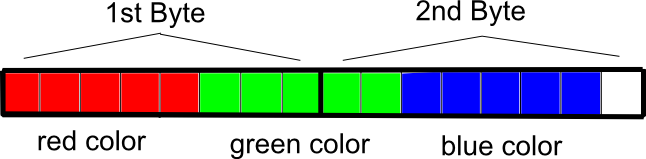
\includegraphics[width=130mm]{Text/IMG/ImageStoring_16bit.png}
	\end{center}
	\caption{A distribution of 16 bits of 2 bytes among three colors of a pixel.}
	\label{screenshot}
\end{figure}

\section{Image enhancement operations}
\label{brightnesscontrast}

One of important tasks to reimplement in Dicom-Presenter was an ability to adjust image brightness and contrast. Images which will be opened in Dicom-Presenter can be captured on various MRI units with various imaging properties. The ability to increase image brightness and contrast is mandatory to ensure sufficient display quality. Too dark or too gray images need to be brightened or need to increase contrast to ensure better observation of physiological findings. A brightness and contrast change is among DICOM users called ``windowing''.

For further needs of this text let's define brightness and contrast. 

A grayscale image can be considered as a matrix of numbers: 

\[
 Im_{res_{x},res_{y}} =
 \begin{pmatrix}
  Im(1,1) & Im(1,2) & \cdots & Im(1,res_{x}) \\
  Im(2,1) & Im(2,2) & \cdots & Im(2,res_{x}) \\
  \vdots  & \vdots  & \ddots & \vdots  \\
  Im(res_{y},1) & Im(res_{y},2) & \cdots & Im(res_{y},res_{x})
 \end{pmatrix}
\]

where $ res_{x} $, $res_{y}$ are dimensions of the image. $Im(x,y)$ is a lightness of a pixel.

Brightness then can be defined as:
\[
  Brightness(Im) = \frac{1}{res_{x}  \cdot res_{y}}\sum_{\substack{0 \leq x \leq res_{x} \\ 0 \leq y \leq res_{y}}} Im(x,y)
\]

Contrast is understood as overall difference in luminosity between bright and dark pixels. There are more possible definitions of contrast. One possible definition is:

\[
Contrast(Im) = \sqrt{\frac{1}{res_{x} \cdot res_{y}}\sum_{\substack{ 0 \leq x \leq res_{x} \\ 0 \leq y \leq res_{y} }}(Im_{x,y}-Brightness(Im))^2}
\]

An argument for using these two definitions for brightness and contrast is that they are analogies for mean value and variance of set of values.

If there is a need of increasing or decreasing image brightness in computer applications simply a constant id added to all image points:

\begin{equation}
\label{brightness}
  Im(x,y) \longmapsto Im(x,y) + c_{brightness} 
\end{equation}

Image contrast is usually adjusted by a linear transformation applied to all image points:

\begin{equation}
\label{contrast}
  Im(x,y) \longmapsto   (Im(x,y) - 0.5) \cdot c_{contrast} + 0.5
\end{equation}

A disadvantage of both ways is that some image information is lost. Let's consider an image described by a matrix with elements of integers in range from zero to 255. Let the brightness of the picture increased according to formula \eqref{brightness} with a positive constant $ c_{brightness} $. Then all the points brighter than $ 255 - c_{brightness} $ on original image will have luminosity of 255 regardless their original luminosity. Similarly if contrast would be increased according to formula \eqref{contrast} with a constant $ c_{contrast} $ then all points brighter than $ \frac{1}{2} \cdot 255 \cdot (\frac{1}{c_{contrast}}+1) $ will have the same color (maximum white). As well all pixels darker than $ \frac{1}{2} \cdot 255 \cdot (1 - \frac{1}{c_{contrast}}) $ will have the same color (maximum black).

\clist{krivka na nelinearni kontrast z vyzkumaku}

\subsection{Pixel manipulations in Qt}

Qt library doesn't offer its own functions for elementary pixel manipulations such as change of brightness and contrast. These operations (described in Section \ref{brightnesscontrast}) must be done in application source code for each image pixel.

A change of brightness or contrast of an image of $m \cdot n$ pixels will be done in $m \cdot n$ steps. In each step a color of the pixel must be obtained, new color value will be calculated and the value will be saved into the picture. Qt library offers two ways to perform the task: pixel manupulation functions or direct memory access.

If preimplemnted Qt pixel manipulation functions are used, the source code will be following:

\begin{lstlisting}[label=qtcontrast,caption={Image enhancement operations implementation using Qt library functions for pixel manipulation.},escapeinside={@}{@}]
QImage image(...);
for (int y=0; y<height; y++) {
	for (int x=0; x<width; x++) {
		@\label{lst:pixel}@QRgb color = image.pixel(x,y);
		@\label{lst:operation}@QRgb newcolor = qRgb(func1(qRed(color)),func2(qGreen(color)),func3(qBlue(color)));
		@\label{lst:setPixel}@image.setPixel(x,y,color);
	}
}
\end{lstlisting}

Function \clist{QRgb QImage::pixel(int x,int y)} is used to retrieve color information of a pixel. The code on line \ref{lst:operation} performs a color manipulation. Function \clist{void QImage::setPixel(int x,int y,QRgb rgb)} is used to save the color information back to the picture. Due to multi-thread programming support the \clist{QImage::setPixel} function offers low performance. Within each function call Qt library must attach and deatach a process to shared memory segment where the image data are stored. These steps are performance expensive.

Nevertheless, Qt library offers a high performance option to change image pixel data. Image data are modified directly inside the computer memory without a function call from QImage class. A function from QImage class is called just to retreive a pointer to memory segment containing image data. The code will be following:

\begin{lstlisting}[label=qtcontrast,caption={Image enhancement operations implementation using Qt library functions for pixel manipulation.},escapeinside={@}{@}]
QImage image(...);
for (int y=0; y<height; y++) {
	@\label{lst:pixel}@QRgb* imageLine=(QRgb*)image.scanLine(y);
	@\label{lst:for}@for (int x=0; x<width; x++) {
		@\label{lst:qrgb}@imageLine[x] = qRgb(func1(qRed(imageLine[x])),func2(qGreen(imageLine[x])),func3(qBlue(imageLine[x])));
	}
}
\end{lstlisting}

Function \clist{QImage::scanLine(int y)} returns a pointer to a segment of memory where is saved \clist{y}-th line of the image. The \clist{QImage::scanLine(int y)} functions returns a pointer to \clist{unsigned char} array (byte array). The conversion to \clist{QRgb} array together with using Qt functions for changing pixel data (line \ref{lst:qrgb}) will remove nescessary byte conversions related do pixel data alignment. If working with the \clist{unsigned char} array, data alignment rules must be respected. The for-cycle browsing through each image line (line \ref{lst:for}) would be ranged to \clist{2*width}, which is actually the real size of an image line in computer memory (expressed in bytes at 16-bit color depth).


\section{Image rendering}



\red{
Renderovani snimku na ruzna mista na obrazovce pomoci Qt.\\
Ukazat bezpecny zpusob pomoci Qt.\\
Ukazat nebezpecny zpusob pomoci primych zasahu do pameti.\\
Zduvodnit proc se radeji priklonime k prehlednemu a bezpecnemu zpusobu pomoci Qt.\\
Zpisob primeho zapisu do pameti at dela jiny student - je to prace na cca pul roku, ale pujde krasne navazat na moji verzi DP.\\
}

\section{OpenGL and Qt performance}

\red{
Ukazat mereni performance a ukazat vzorecek na odhad rychlosti vykreslovani.\\
}